\glspl{kg} have came up as a key technology in the field of data management and \gls{ai}, enabling sophisticated data integration, retrieval and analysis.
This section provides an in-depth overview of \glspl{kg}, their theoretical foundations, practical applications and recent advances.

\subsection*{Theoretical Foundations of Knowledge Graphs}
\subsubsection*{Definition and Structure}
\glspl{kg} are directed graph-based data structures that represent real-world entities and their interrelations, providing a way to model complex domains and their underlying semantics.
A \gls{kg} consists of nodes (also called entities) and edges (also called relationships), forming a network of interconnected information.
This structure allows \glspl{kg} to capture rich contextual information and provide a semantic framework for data \cite{Hogan2021}.
In other words, a \gls{kg} refers to a semantic network graph which is consisted of diverse entities, concepts, and relationships.
It is used to formally describe various things and their associations in the real world.
\glspl{kg} are generally represented in triples $\gls{kg}=\{\mathnormal{E,R,F}\}$, where:
\begin{itemize}
    \item $E$ represents the entity set $\{\mathnormal{e_1, e_2, ... ,e_E} \}$, and the entity $e$ is the most basic element in the \gls{kg}, referring to the items that exist objectively and can be distinguished from each other.
    \item $R$ represents the relation set $\{\mathnormal{r_1, r_2, ... ,r_R}\}$, and the relation $r$ is an edge in the \gls{kg}, representing a specific connection between different entities.
    \item $F$ represents the fact set $\{\mathnormal{f_1,f_2, ... ,f_F}\}$, and each $\mathnormal{f}$ is defined as a triple $(\mathnormal{h,r,t}) \in \mathnormal{f}$, in which $\mathnormal{h}$ denotes the head entity, $\mathnormal{r}$ stands for the relationship, and $\mathnormal{t}$ indicates the tail entity.
\end{itemize}

The \gls{kg} in Fig.~\ref{fig:kg-example-albert-einstein} visually represents some relationships and attributes associated with Albert Einstein.

\begin{figure}[htbp]
    \centering
 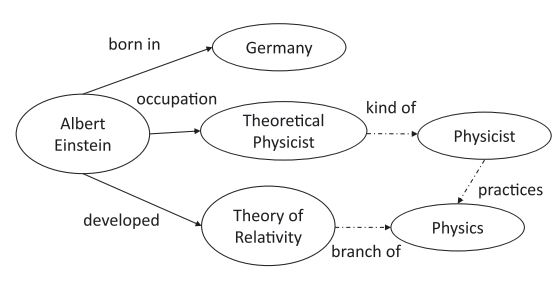
\includegraphics[width=.8\textwidth]{figures/literature-review/kg-example-albert-einstein.png}
     \rule{35em}{0.5pt}
    \caption{An example of \acrlong{kg} (\textcite{Chaudhri2022})} 
 \label{fig:kg-example-albert-einstein}
\end{figure}

At the center of the graph is ``Albert Einstein'', from which several connections extend.
One connection indicates that he was ``born in'' Germany.
Another connection shows his ``occupation'' as a ``Theoretical Physicist''.
This occupation is further connected to ``Physicist'' as a ``kind of'' category, indicating that a theoretical physicist is a type of physicist.
The graph also shows that a physicist ``practices'' physics.
Additionally, it highlights that Albert Einstein ``developed'' the ``Theory of Relativity'', which is shown as a ``branch of'' physics.
The graph effectively maps out key aspects of Albert Einstein's background, profession, and contributions to science.

\subsubsection*{Ontologies and Semantic Web Technologies}
An ontology is a formal representation of knowledge in a domain, specifying the concepts, relationships, and constraints that exist within that domain. The term ``ontology'' can be used to the shared understanding of some domain of interest \cite{Uschold1996}.
Ontologies play a critical role in defining the schema and semantics of \glspl{kg}. They specify the types of entities, relationships, and constraints, thereby providing a formalized structure for the data. The Semantic Web technologies, particularly the \gls{rdf} and the \gls{owl}, are fundamental to the development and functioning of \glspl{kg} \cite{Antoniou2008}.
\\\gls{rdf} is a standard model for data interchange on the web.
\gls{rdf} is a part of the \gls{w3c}'s Semantic Web activity and provides a model for data interchange on the Web.
It uses triples $\langle subject,predicate,object \rangle$ to represent information, providing a flexible and extensible framework for creating and managing \glspl{kg} \cite{Cyganiak14RCA}.
The subject is the resource being described, the predicate is the property or characteristic of the subject, and the object is the value of the property, that can be literals, which are concrete data values such as strings, numbers, or dates.
\gls{rdf} uses \glspl{uri} to uniquely identify subjects and predicates, ensuring that resources are globally identifiable.
\gls{rdf} can be serialized in various syntaxes, including \gls{rdf}/XML, Turtle, N-Triples, and JSON-LD. \gls{rdf}/XML is the original \gls{rdf} syntax using XML to represent \gls{rdf} triples. Turtle is a more human-readable syntax for \gls{rdf} data, concise and easier to write and read compared to \gls{rdf}/XML. N-Triples is a plain text format for encoding \gls{rdf} triples, useful for streaming data or simple data exchange. JSON-LD is a JSON-based format to serialize Linked Data, designed to be easy to use and integrate with existing JSON-based systems.

\gls{rdfs} is a semantic extension of \gls{rdf} that provides mechanisms to describe groups of related resources and the relationships between these resources. It allows for defining classes, which are categories of resources; properties, which are relationships between resources; and hierarchies, enabling inheritance.
\gls{rdf} is widely used in various domains, including the Semantic Web, where it enables the creation of a web of data with meaning, allowing machines to understand and process web content; \glspl{kg}, powering large-scale graph-based data structures used by organizations like Google and Amazon \cite{Kejriwal2022}; data integration, integrating data from disparate sources by providing a common data model; and ontology engineering, defining and using ontologies to model domain knowledge.

The \gls{owl} standard is a \gls{w3c} technology for defining and using web ontologies, enhancing \gls{rdf} by offering greater expressiveness for complex information. \gls{owl} ontologies consist of classes, properties, and individuals, enabling detailed descriptions of relationships and characteristics. It supports complex class expressions, including logical operators and restrictions like cardinality and property constraints.
\gls{owl} is used to explicitly represent the meaning of terms in vocabularies and the relationships between those terms. It enables more complex and expressive representations compared to \gls{rdfs} \cite{Deborah2004}.
\gls{owl} is used in knowledge management, information integration, and semantic search, providing a common framework for understanding and integrating data. It promotes interoperability and the creation of semantically rich, interconnected web data.

\subsubsection*{Query Languages}
\gls{sparql} is the standard query language for retrieving and manipulating data stored in \gls{rdf} format.
This query language is used to retrieve data from the GraphDB\footnote{\url{https://www.ontotext.com/products/graphdb/}} database.
It allows users to write complex queries to extract specific information from a \gls{kg}, making it a powerful tool for data analysis and knowledge discovery \cite{Jorge2009}.
It allows users to query \gls{rdf} data by specifying patterns of triples and to update \gls{rdf} data by inserting, deleting, and modifying \gls{rdf} triples.
\gls{rdf} is a foundation for \gls{lod}, which involves interlinking data across the web using \glspl{uri} and \gls{rdf}. This enables the creation of a web of data that can be easily connected and queried.

Cypher is another query language for graph databases, such as Neo4j\footnote{\url{https://neo4j.com}}, that allows users to interact with graph data using a pattern-matching syntax. Cypher queries are used to traverse the graph, retrieve specific patterns, and perform operations on the data \cite{Francis2018}.
Cypher supports complex queries involving multiple nodes and relationships, aggregation, sorting, and limiting results. It also provides functions for working with strings, numbers, dates, and collections, as well as support for subqueries and variable-length paths.
Cypher is widely used for graph analytics, network analysis, and data exploration, enabling users to easily express complex graph traversals and operations. It leverages Neo4j's indexing and optimization capabilities to ensure efficient execution of queries, making it a powerful tool for working with connected data.

\subsection*{Applications of Knowledge Graphs}

\subsubsection*{General Applications}
\glspl{kg} have been adopted across various domains due to their ability to integrate heterogeneous data sources, provide semantic context, and enable advanced querying and reasoning.
According to \textcite{Kapanipathi2020}, in healthcare \glspl{kg} are used to integrate patient records, clinical trials, research data, and medical ontologies, enabling personalized medicine and decision support systems. They help in identifying relationships between diseases, treatments, and patient outcomes.
\\Financial institutions leverage \glspl{kg} to connect data from various sources, such as market data, regulatory information, and customer transactions. This integration facilitates risk management, fraud detection, and compliance monitoring \cite{Tchechmedjiev2019}.
\\In e-commerce, \glspl{kg} enhance product recommendation systems by linking customer preferences, purchase history, and product information. They enable more personalized and relevant recommendations, improving customer satisfaction and sales \cite{Zhang2021}.

In compliance with \textcite{Zou2020}, Fig.~\ref{fig:kg-application-fields} shows a mind map illustrating the main applications of knowledge graphs. It divides the applications into five main categories: question answering, recommendation systems, information retrieval, domain-specific applications and other applications.

\begin{figure}[htbp]
    \centering
 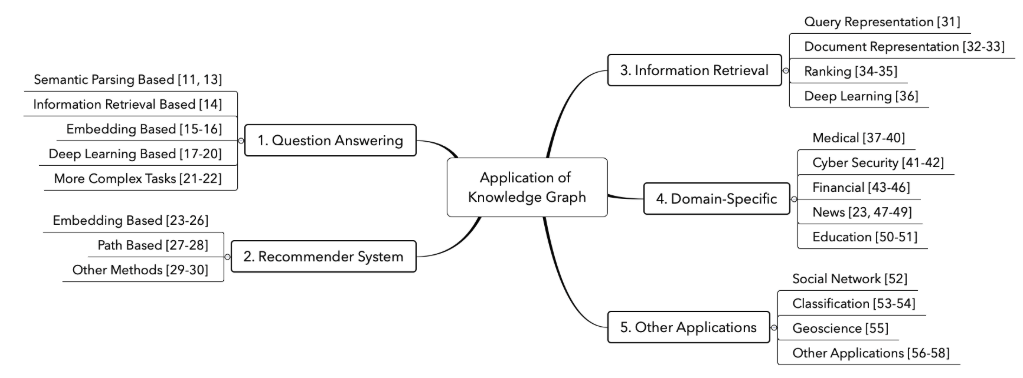
\includegraphics[width=.92\textwidth]{figures/literature-review/kg-application-fields.png}
     \rule{35em}{0.5pt}
    \caption{Application of \acrlongpl{kg} (\textcite{Zou2020})} 
 \label{fig:kg-application-fields}
\end{figure}

With regard to question answering, methods based on semantic parsing, methods based on information retrieval, methods based on embedding, methods based on \gls{dl} and more complex tasks are included.
\glspl{kg} significantly enhance search engines by providing semantic search capabilities. They enable the understanding of user queries in context, allowing for more accurate and relevant search results. Google's Knowledge Graph is a prominent example, enhancing search results with information about entities and their relationships \cite{singhal2012introducing}.
Recommender systems are classified into embedding-based methods, path-based methods and other methods. Information retrieval includes query representation, document representation, ranking and \gls{dl}. Domain-specific applications include medicine, computer security, finance, news and education.
Within enterprises, \glspl{kg} are used to manage and utilize internal knowledge effectively. They integrate data from different departments, such as human resources, finance, and operations, providing a unified view of the organization's information. This integration supports decision-making, collaboration, and innovation \cite{pujara2013knowledge}.
Other applications include social networks, classification, geosciences and various other applications.


\subsection*{Recent Advancements in Knowledge Graphs}

\subsubsection*{Integration with Machine Learning}
Recent research has focused on integrating \glspl{kg} with \gls{ml} and \gls{dl} techniques to enhance their capabilities and applications. These integrations have led to significant advancements in various areas, including \gls{nlp}, recommendation systems, and predictive analytics.

\glspl{kge}: \gls{kge} techniques represent entities and relationships in a continuous vector space, enabling the use of \gls{ml} algorithms for tasks such as link prediction, entity classification, and clustering. Popular methods include TransE \cite{Bordes2013}, TransH \cite{Wang2014}, and TransR \cite{Lin2015}, each providing different ways to model relationships in the embedding space \cite{Wang2017}.

\glspl{gnn}: \glspl{gnn} are \gls{dl} models designed to operate on graph-structured data. They leverage the relational nature of graphs to perform tasks such as node classification, link prediction, and graph classification. \glspl{gnn} have been successfully applied to enhance the capabilities of \glspl{kg} in various domains \cite{Wu2021}.

\subsubsection*{Natural Language Processing and Question Answering}
\glspl{kg} have been instrumental in advancing \gls{nlp} applications, particularly in question answering systems. By providing structured and semantically rich information, \glspl{kg} enable systems to understand and generate human language more effectively.
\glspl{kg} support question answering systems by enabling them to retrieve and reason over structured data.
These systems can answer complex queries by traversing the graph and applying logical inferences based on the relationships between entities \cite{Yasunaga2021}.
\glspl{kg} enhance text analysis and semantic search by providing contextual information about entities mentioned in the text.
This contextual understanding improves the accuracy of information retrieval and the relevance of search results \cite{Fernandez2011}.

\subsection*{Well-Known Knowledge Graphs and Ontologies in Research Field}
Well-known \glspl{kg} and ontologies have significantly influenced the research field by providing structured representations of knowledge that facilitate data integration, retrieval, and analysis.
One prominent example was the \gls{mag}, a comprehensive dataset that mapped scholarly publications, authors, institutions, and topics, enabling advanced research trend analysis and collaboration discovery \cite{Wang2020}.
Although \gls{mag} was discontinued in 2021 as Microsoft shifted its focus to supporting open academic initiatives, its legacy lives on through platforms like OpenAlex, a successor to \gls{mag} that serves as an open-source resource connecting entities such as authors, publications, and journals with detailed metadata \cite{priem2022}.

\begin{figure}[htbp]
    \centering
 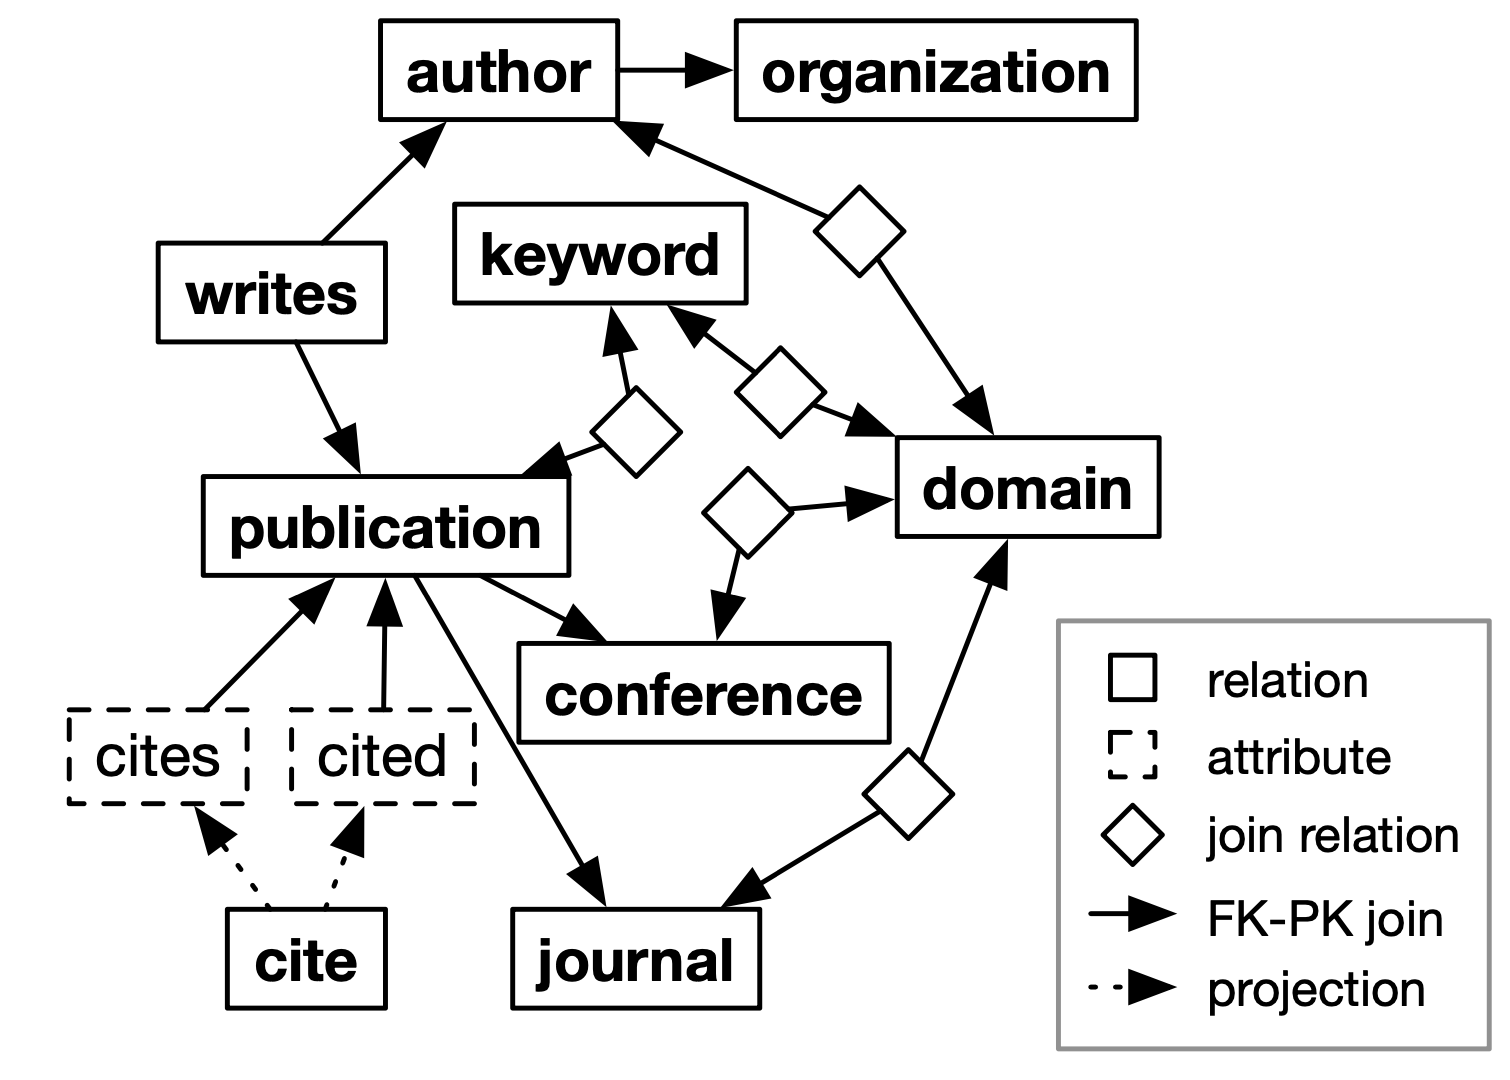
\includegraphics[width=.6\textwidth]{figures/literature-review/mag-schema.png}
     \rule{35em}{0.5pt}
    \caption{A simplified version of the \gls{mag} Search database's schema (\textcite{Baik2019})} 
 \label{fig:mag-schema}
\end{figure}

Another essential resource is the the \gls{s2ag}, developed by the Allen Institute for \acrlong{ai}, represents one of the most extensive and advanced knowledge graphs in the research domain \cite{S2AG}.
\gls{s2ag} contains over 205 million publications, 121 million authors, and nearly 2.5 billion citation edges, making it a powerful resource for understanding and analyzing academic networks.
By integrating metadata from sources such as Crossref, PubMed, and Unpaywall, and processing nearly 60 million full-text publications, \gls{s2ag} enables rich insights into scholarly communication.
The data is accessible through public APIs and downloadable snapshots, fostering applications in natural language processing, citation analysis, and research trend discovery.
\gls{s2ag} exemplifies the potential of \glspl{kg} to address information overload by enabling efficient discovery of relevant research literature.
Its availability as an open resource highlights the growing emphasis on open science and collaborative innovation in the academic community.

Wikidata is a collaboratively edited \gls{kg} that serves as a centralized data repository for structured information across various domains, supporting Wikimedia projects like Wikipedia and numerous external applications \cite{Wikidata2014}.
Introduced in 2012 by the Wikimedia Foundation, Wikidata provides a platform where entities, such as people, places, events, and concepts, are represented as items with unique identifiers.
These items are described using statements, which consist of properties and values, forming a triple-based structure similar to other semantic web technologies.
One of the most distinguishing features of Wikidata is its adherence to the principles of \gls{lod}.
It allows the integration with other \glspl{kg} and ontologies by supporting globally recognized identifiers, such as \glspl{doi}, \glspl{orcid}, and \gls{viaf} IDs, and linking to external datasets.
This capability makes it a valuable resource for connecting fragmented knowledge across the web.
The Wikidata \gls{kg} is highly dynamic and continuously enriched by a global community of contributors and automated tools like bots.
Its multilingual support ensures accessibility to a diverse audience.
Applications of Wikidata include natural language processing, recommendation systems, semantic search, and research in \gls{ai}.
Due to its openness, flexibility, and integration capabilities, Wikidata is increasingly being adopted as a foundational resource for creating and enriching domain-specific knowledge graphs, supporting scholarly projects, and powering data-driven insights.

Furthermore, the \gls{orkg} offers a dynamic, semantic representation of research contributions, focusing on contextualizing findings within their scientific domain to support comparative studies and systematic reviews \cite{ORKG}.
The \gls{orkg} aims to address the challenge of information overload in scholarly research by structuring and presenting scientific knowledge in a machine-readable format.
Unlike traditional research dissemination approaches, which rely on static publications, the \gls{orkg} provides a platform for collaboratively curating research content with semantically rich metadata, enabling advanced analysis and discovery.
Through the use of \gls{lod} principles and Semantic Web technologies, the \gls{orkg} facilitates the comparison of research findings across studies by aligning key concepts, methodologies, and outcomes.
This structured representation allows researchers to identify gaps in the literature, reproduce experiments, and generate new insights with greater efficiency.
The platform also supports automated reasoning and \gls{ai}-driven tools, making it easier to navigate large volumes of data and extract relevant patterns or trends.
The \gls{orkg} is particularly valuable for interdisciplinary research, where integrating knowledge from multiple domains is essential.
By linking related studies and establishing semantic connections between concepts, the \gls{orkg} enhances the accessibility and usability of scientific knowledge for both humans and machines.
This approach not only accelerates scientific progress but also lays the groundwork for the next generation of research infrastructures.

The VIVO Ontology, which forms the core of the VIVO platform and is designed to represent scholarly activity in a structured and interoperable manner \cite{VIVO}.
It emphasizes the use of semantic technologies such as \gls{rdf} and \gls{owl} to model relationships among academic entities like researchers, publications, grants, and institutions.
By employing these standards, the ontology enables data to be expressed in a machine-readable format as triples, which facilitates reasoning, integration, and discovery.

\begin{figure}[htbp]
    \centering
 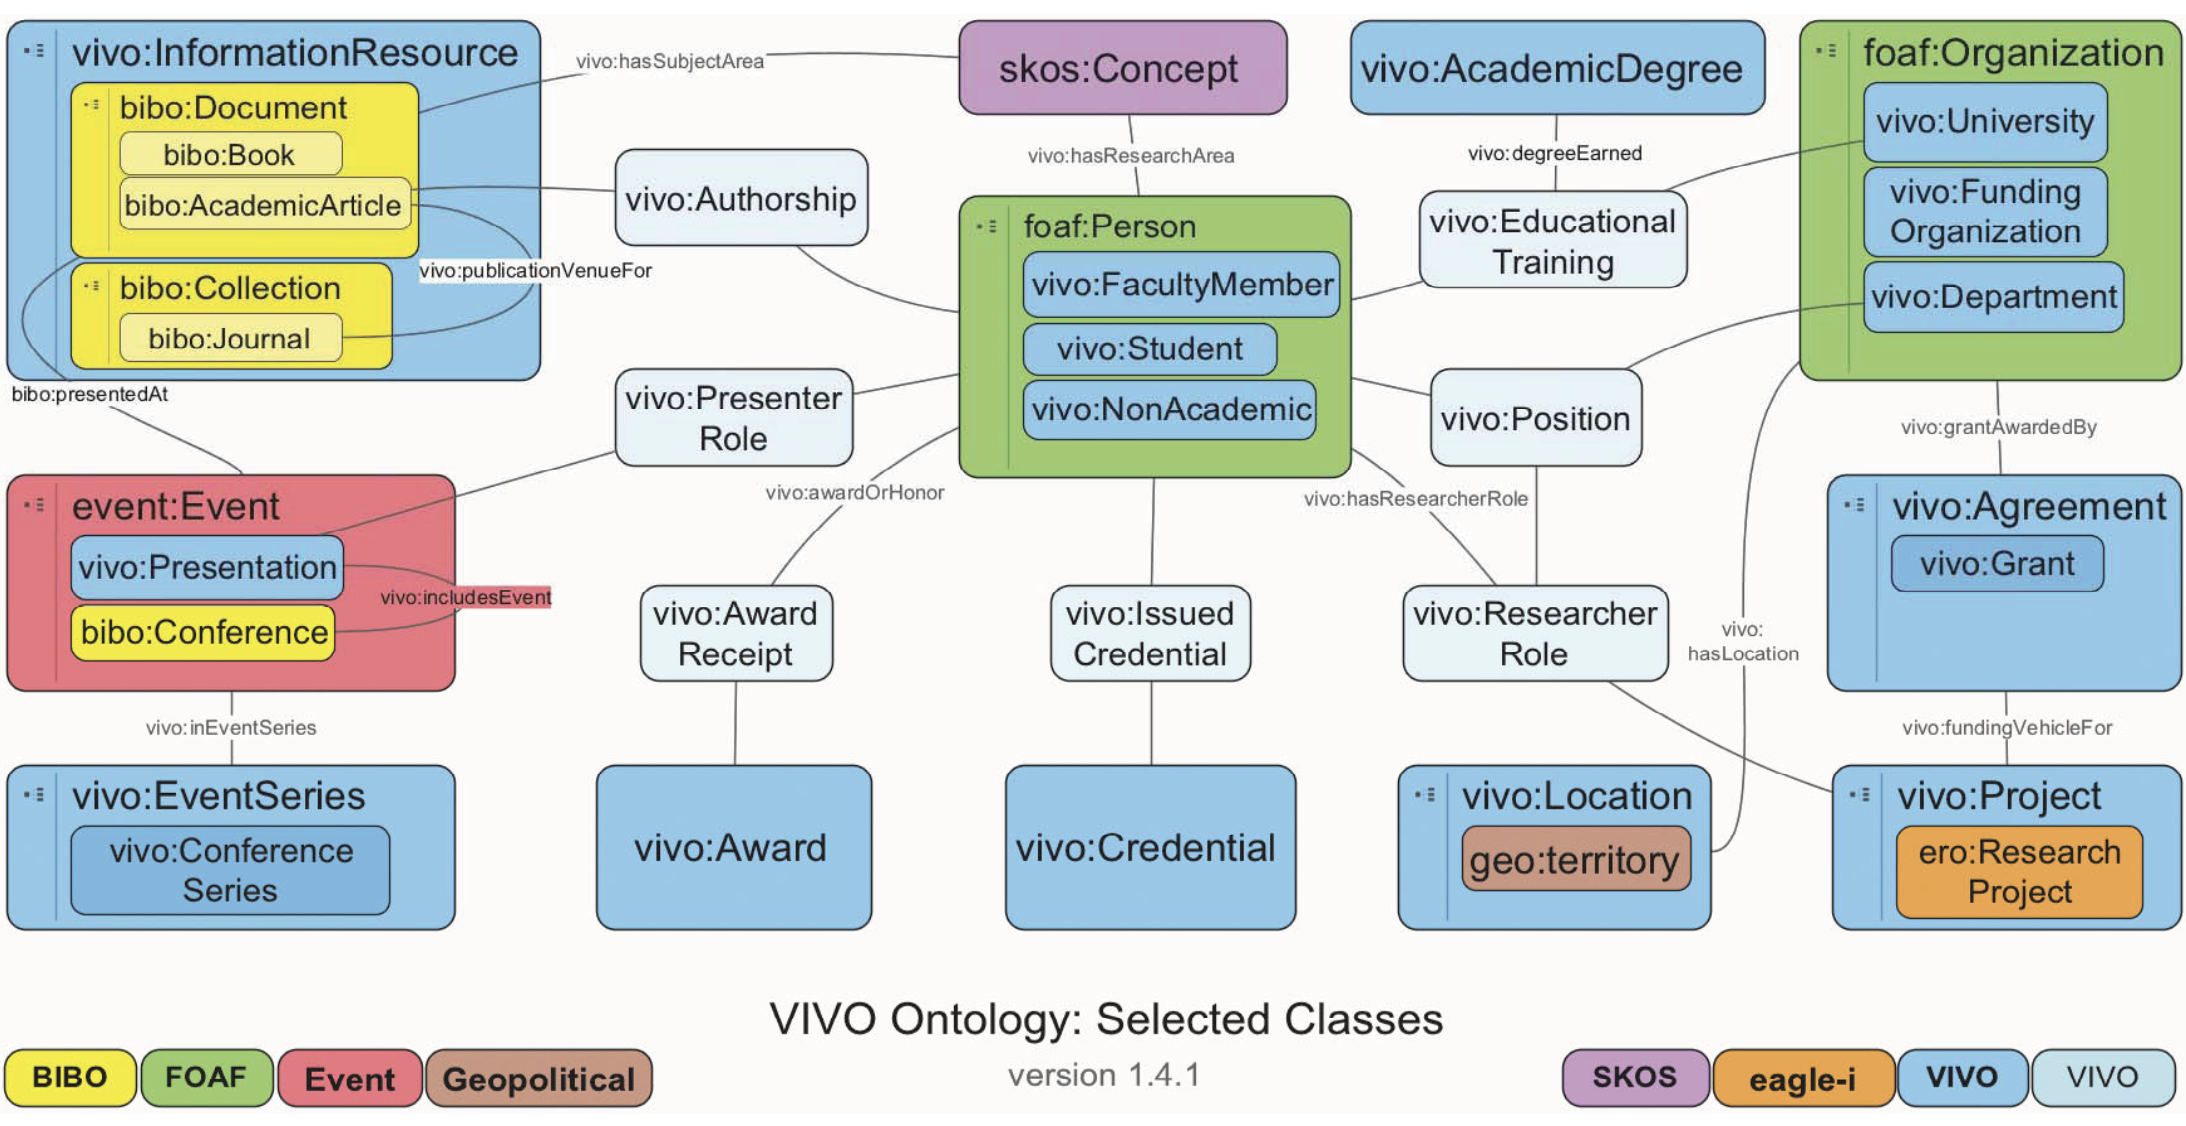
\includegraphics[width=.9\textwidth]{figures/literature-review/vivo-ontology.png}
     \rule{35em}{0.5pt}
    \caption{Key classes in the VIVO ontology are highlighted alongside their source ontologies, with ``context nodes'' (depicted in light blue) providing temporal details and other information specific to individual relationships. (\textcite{VIVO})}
 \label{fig:vivo-ontology}
\end{figure}

The design of the VIVO Ontology is guided by clear goals, including the ability to represent complex academic relationships and maintain independence from specific implementations to ensure adaptability across diverse institutional contexts.
A hierarchical class structure is employed to define scholarly entities, with an emphasis on modularity and scalability to accommodate the evolving needs of the academic community.
Additionally, the ontology supports the use of external controlled vocabularies and common identifiers to enhance data consistency and interoperability with other systems.

VIVO leverages several well-established ontologies, such as \gls{foaf}, to enrich its representation of scholarly data and ensure interoperability with other systems.
\gls{foaf} is a widely-used ontology designed to describe people, their activities, and their relationships to other people and objects.
The core element of a \gls{foaf} document is the \gls{foaf} vocabulary, which is defined by the namespace: \textless http://xmlns.com/foaf/0.1/\textgreater.
By integrating \gls{foaf}, VIVO can represent entities like researchers and their social networks, enabling a consistent and standard framework for modeling relationships such as collaborations, affiliations, and connections to digital artifacts like websites or profiles.
The primary reason VIVO uses \gls{foaf} is to adopt existing, well-defined vocabularies rather than reinventing the wheel, which promotes interoperability across systems and facilitates data sharing on the Semantic Web.
\gls{foaf}'s compatibility with \gls{lod} principles allows VIVO to easily connect its data with external resources, enhancing discoverability and integration.
For example, \gls{foaf}'s properties such as foaf:Person and foaf:knows align perfectly with VIVO's requirements for describing researchers and their relationships, while maintaining compliance with Semantic Web standards.
By utilizing external ontologies like \gls{foaf}, VIVO not only achieves a more robust and extensible data model but also ensures that its ontology can interact with broader data ecosystems, advancing the goal of creating a globally connected research information infrastructure.
This strategic reuse of established ontologies supports VIVO's vision of openness, interoperability, and scalability in scholarly networking and discovery.
The VIVO Ontology serves as the core of the VIVO application, functioning as a data model and enabling reasoning to infer new relationships based on existing data.
Its flexibility allows institutions to extend the ontology to meet specific local requirements while adhering to its core principles, thereby maintaining compatibility with the broader VIVO ecosystem.
Community-driven efforts play a crucial role in the continuous refinement and expansion of the ontology, ensuring its relevance and alignment with advancements in academic practices.
By supporting the creation of \gls{lod}, the VIVO Ontology facilitates improved research discovery, expert identification, and collaboration across institutions.